\documentclass[10pt]{article}
\usepackage[hmargin=1.25cm, vmargin=1.5cm]{geometry}
\usepackage{bbding}
\usepackage{multirow}
\usepackage{amssymb}
\usepackage{eurosym}
\usepackage{color,graphicx}
\usepackage[usenames,dvipsnames]{xcolor}
\usepackage{fontspec,xltxtra,xunicode}
\defaultfontfeatures{Mapping=tex-text}
\setromanfont[Mapping=tex-text]{Hoefler Text}
\setsansfont[Scale=MatchLowercase,Mapping=tex-text]{Gill Sans}
\setmonofont[Scale=MatchLowercase]{Andale Mono}
\DeclareGraphicsExtensions{.pdf,.png,.jpg}
%Setup hyperref package, and colours for links, text and headings
\usepackage{hyperref}
%\definecolor{linkcolor}
%{HTML}{FF0080} %light purple link for the email
\definecolor{linkcolor}{HTML}{00008B}
\definecolor{shade}{HTML}{D4D7FE}      %light blue shade
%\definecolor{text1}{HTML}{2b2b2b}      %text is almost black
\definecolor{text1}{HTML}{000000}      %text is black
\definecolor{headings}{HTML}{00008B}   %navy blue
\hypersetup{   colorlinks,breaklinks,
               urlcolor=linkcolor,
               linkcolor=linkcolor
}

\usepackage{fancyhdr}                  %custom footer
\pagestyle{fancy}
\fancyhf{}
\rfoot{\small\color{headings} {\sffamily Last update: \today}. 
Typeset with X\LaTeX}
\renewcommand{\headrulewidth}{0pt}

\usepackage{titlesec}                  %custom \section

\titleformat{\section}
   {\color{headings}
      \scshape\Large\raggedright}{}{0em}{}[\color{black}\titlerule]

\titlespacing{\section}{0pt}{0pt}{3pt}

\begin{document}
\color{text1} % set text color for the whole doc
     \par{\centering{\sffamily\huge Joseph Randall Hunt}\\
      \color{headings}\fontspec[Variant = 2]{Zapfino} Curriculum 
      {Vit\fontspec[Variant = 3]{Zapfino}\ae}\\[25pt]\par
      %\color{headings}\fontspec[Variant = 2]
      %{Zapfino}R\'esum\'e\\[20pt]
      {\color{white} \hrule}} %does this rule really change anything?

\begin{minipage}[t]{0.5\textwidth}

\vspace{0pt}   %trick

\section{Work Experience}
   \raggedleft
   \textsc{\normalsize January 2011 -- May 2011}\par
   \raggedright\large Undergraduate Researcher\\
   \textsc{NASA Ames Research Center}\\
   \normalsize{Created an Automatic KML Tour Generator and KML Tour 
   Editor using Django, Python, SQL, and Javascript. Media import tool
   pulls from several different sources and loads all data into a 
   database. Project generated a whole new set of data products for
   the Maps team.}\\[5pt]

   \raggedleft
   \textsc{\normalsize August 2010 -- December 2010}\par
   \raggedright\large Academic Engagement and IT Governance\\
   \textsc{Western Carolina University}\\
   \normalsize{Resolved IT issues involving several topics from 
   networking to software configuration. Also taught several 
   workshops on web development.}\\[5pt]

   \raggedleft
   \textsc{\normalsize June 2010 -- August 2010}\par
   \raggedright\large Undergraduate Researcher\\
   \textsc{NASA Langley Research Center}\\
   \normalsize{Worked on several tools for mass properties evaluation
   which culminated in the design a mass properties API. Also worked
   with an 8 person team to design and evaluate a series of tests on
   a flotation concept. If implemented project could save millons of
   dollars. Findings were published to NASA's main webpage, AIAA 
   newsletter, and several other notable websites.}\\[5pt]

   \raggedleft
   \textsc{\normalsize August 2009 -- June 2010}\par
   \raggedright\large Lab Admin and Teaching Assistant\\ 
   \textsc{Western Carolina University}\\
   \normalsize{Assisted professor and students in an undergraduate 
   computer science course. Maintained the computer science lab 
   computers running Linux, Windows, and OSX with several VMs.
   Created scripts to automatically update all computers and all VMs.
   Managed backups leading to a \%5 decrease in downtime.}\\[5pt]

\section{\textsc{Technical Skills}}
   \begin{tabular}{rl}
      \textbf{\textsc{Languages}}:
                        & \textbf{Professional}:\\
                        & Java, C, Python, (My,Postgre)SQL,\\
                        & HTML/CSS/Javascript, XML\\
                        & \\
                        & \textbf{Familiar}:\\
                        & Scheme (Lisp), PHP, C++\\
                        & Perl, Prolog, Objective-C\\
                        & \\
      \textbf{\textsc{Frameworks}}:
                        & Cocoa, jQuery, Wordpress, Django\\
                        & \\
      \textbf{\textsc{Tools}}:
                        & Eclipse, Mathematica, Labview,\\
                        & XCode, ViM, ant, jUnit\\
                        & \\
      \textbf{\textsc{Mathematics}}:
                        & Formal Logic and Proof Techniques,\\
                        & Linear Algebra, Calculus,\\
                        & Statistics, Discrete Structures\\
\end{tabular}
\end{minipage}
\hfill
\begin{minipage}[t]{0.44\textwidth}

   \vspace{-10pt} %trick for alignment
\colorbox{shade}{\textcolor{text1}{
      \begin{tabular}{c|p{4.25cm}r}
                                    %Can't include this in a lot of forms.
                                    %& Born in North Carolina in 1991\\
         \raisebox{-1pt}{\Phone}    &+1(650) 690-0657
         &\raisebox{2.9pt}{\multirow{2}{*}{
             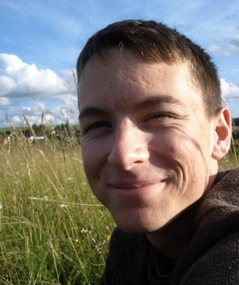
\includegraphics[height=1.45cm]{randall}
             }}\\ 
         \raisebox{-1pt}{\textsc{www}} &
         \href{http://www.jrhunt.org/}{www.jrhunt.org}&\\
         \raisebox{-3pt}{\Envelope} &
         \href{mailto:randall.hunt@gmail.com}{randall.hunt@gmail.com}& 
      \end{tabular}
    }
}\\[3pt]

\section{Education}
\begin{tabular}{rl}
   \textsc{May} 2012 & B.S. in \textsc{Computer Science and Math}\\
      & \textbf{Western Carolina University}\\
      %& Major GPA: \textbf{3.67}\\
      & Cullowhee, NC\\
      &\\
   \textsc{June} 2009 & High School\\
      & \textbf{Punahou Academy}\\
      & Honolulu, Hawaii\\
      &\\
   \textsc{Summer} 2007 & Certificate of Proficiency in French\\
      & \textbf{Université Catholique De L'Ouest}\\
      & Angers, France\\
\end{tabular}\\[5pt]

\section{Languages}
\begin{tabular}{rl}
   \textsc{French}   &  Proficient\\
   \textsc{German}   &  Conversational\\
   \textsc{Russian}  &  Basic\\
   \textsc{Spanish}  &  Learner\\
\end{tabular}\\[5pt]

\section{Activities and Societies}
   IEEE Member\\
   \href{http://polaris.cs.wcu.edu/~acm/}{Student ACM Chapter}\\
   \href{https://github.com/ranman}{Open-Source Contributor}\\
   Active on \href{http://stackoverflow.com/users/240004/ranman}
   {StackOverflow}\\
   Passionate about Robotics\href{http://robotics.punahou.edu/}{[1]}
   \href{http://irg.arc.nasa.gov}{[2]}\\
   \href{http://www.youtube.com/user/ranman96734}{Rubik's Cubes}\\
   \href{http://www.punahouaquatics.org/Home.jsp?team=hipaq}
   {Love to Surf and Swim}\\
\section{Coursework}
   Multiuser Chat System in Java\\
   Address Book with RMI in Java\\
   Set Associative Cache Simulator in Java\\
   Tokenizer and Parser in C\\
   Paint Clone in Java\\
   Email Client in Java\\
   Wireless Sensor Grapher in TinyC+Java\\
   TCP Implementation in TinyC\\
   Adventure Game in Prolog\\
\section{Honors}
   Academic Technology Advisory Committee\\
   AP Scholar's Award\\
   Several Presenations at NASA\\
   Dean's List\\
   Honors College\\
\end{minipage}
\end{document}
